\documentclass[11pt]{article}
\usepackage[margin=1in]{geometry}
\usepackage{graphicx}
\usepackage{microtype}
\usepackage{verbatim}
\usepackage{amsmath}
\usepackage{nicefrac}
\usepackage[colorlinks=false, pdfborder={0 0 0}]{hyperref}
\begin{document}
\title{Rudder Controller \& Wiper Controller\\Embedded System Design, Lab 2}
\date{September 25, 2015}
\author{Ben Lorenzetti}
\maketitle
\tableofcontents

\clearpage

\section{Objectives and Problem Description}

The primary objective of this lab was learning to interface with two new types of peripherals: a servo motor and potentiometers.
Several new functions in PBASIC are introduced for these types of actuators and transducers.

\subsection{Rudder Controller}

Control the angular position of a tiny ship's rudder (i.e. the horn of your servo)
based on the input from a steering wheel (i.e. your potentiometer).
The full range of motion of the ship's rudder should be $45^{o}<\theta<135^{o}$
and it should be controlled linearly by the full range of the potentiometer.

\subsection{Wiper Controller}

Instead of controlling angular position, as was done for the rudder controller,
use the potentiometer to control the angular velocity of the servo.
The servo represents a single windshield wiper, and should rotate continuously
between $15^{o}$ and $160^{o}$. The full range of the potentiometer should
be used to linearly control the wiper speed from 0 degrees/sec up to the
maximum speed.

\section{Procedure}
\subsection{Assignment: Ch. 4 Servo Motor}

To prepare for this lab, we were instructed to read chapters 4 and 5 in the Parallax What's a Microcontroller book and complete the example activities.

The parallax servo motor has three connectiong: power, ground, and signal.
The signal (white) connection is used to control the angular position of
the horn, from $0^{o}$ to $180^{o}$.
The servo expects a square wave control signal,
where the period is approximately 20 ms
and the width of the high pulse carries angular displacement information.

\begin{figure}[h!]
\centering
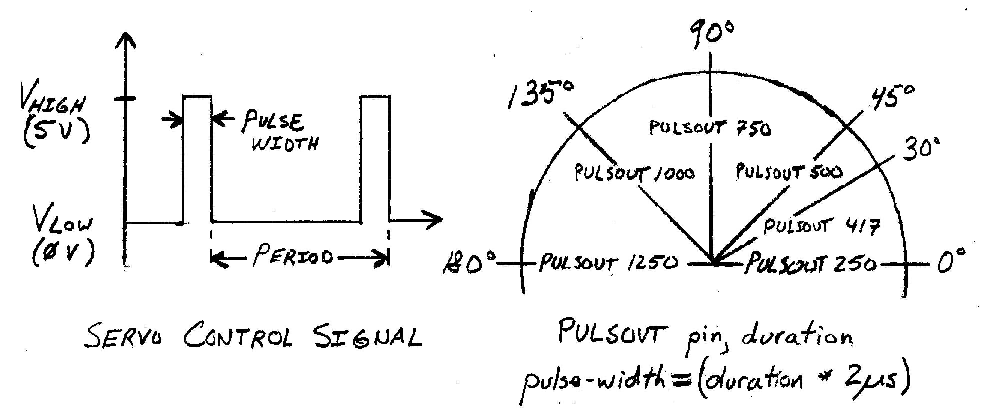
\includegraphics[width=0.8\textwidth]{pulse-width-vs-angular-displacement.pdf}
\caption{Servo Control Signal Timing}
\label{pulse-width-vs-angular-displacement}
\end{figure}

The formula relating pulse width and angular displacement is
\begin{equation}
t_{p-width}(\theta)=\left\{\begin{array}{c c}
\frac{500\mu s}{45^{o}}\theta+500\mu s	&	10^{o}<\theta<170^{o}\\
0\mu s	&	\textrm{servo off}	\\
\end{array}\right.
\label{pulse-width-eq}
\end{equation}

The function for doing pulse width modulation in PBASIC is
\texttt{PULSOUT pin, duration}, where \texttt{pin} is the
I/O port number and \texttt{duration} is the length of time high.
Of course, since this Stamp and PBASIC, the board isn't quite
fast enough so \texttt{duration} is in units of $2\mu s$ and
you have to complete the pulse width modulation yourself by
\texttt{PAUSE}ing for 20 ms, or however long the period should
be approximately.

To avoid dealing with PBASICs strange limitations,
we can rewrite equation \ref{pulse-width-eq} as
\begin{equation}
\textrm{duration}=\frac{50}{9}*\theta+250, \quad 10^{o}<\theta<170^{o}
\end{equation}

Chapter 4 also provided two more expressions in PBASIC that are helpful with servo motors:
\begin{verbatim}
i VAR Word
FOR i = 0 TO 150
	...
LOOP
}
\end{verbatim}
and
\texttt{duration = duration MIN 350 MAX 1150}.

\subsection{Assignment: Ch.5 Potentiometers}

Not surprisingly, the Basic Stamp is too primative to have an analog-to-digital converter,
so you can only measure analog inputs with a function called \texttt{RCTIME},
and then only if you construct an RC decay circuit--and again only if the input
signal is stable for a long enough charging time and can source enough current.

The function prototype is \texttt{RCTIME pin, state, duration},
where \texttt{pin} is the I/O pin number (0-15), \texttt{state} is the
expected charged status of the pin (0 or 1), and \texttt{duration} is
a variable to store the decay time--in units of $2\mu s$.
The decay time is taken when the voltage on \texttt{pin} falls below
$1.4V$, if the original charge \texttt{state} was 1.

\begin{figure}[h!]
\centering
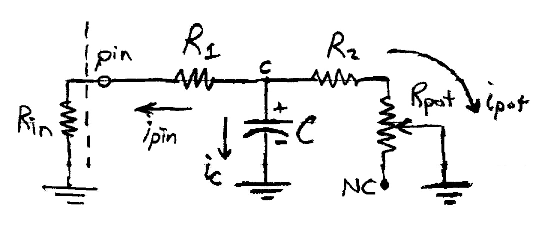
\includegraphics[width=0.5\textwidth]{pot-input-circuit.pdf}
\caption{Input Circuit for Reading a Potentiometer with \texttt{RCTIME}}
\label{pot-input-circuit}
\end{figure}

An input source that is well suited to \texttt{RCTIME} is a rotary
potentiometer. A circuit combining a potentiometer and capacitor is shown
if \hyperref[pot-input-circuit]{figure \ref{pot-input-circuit}}.

If we assume infinite input resistance once \texttt{RCTIME} switches
the pin direction to input, then $i_{pin}=0$ and $V_{in}=V_{c}$.
Taking Kirchoff's Current Law at node c allows us to solve for input
voltage as a function of time and initial condition across C.
\begin{equation*}
i_{pin}+i_{c}+i_{pot}=0
\end{equation*}
\begin{equation*}
0+C\frac{dV_{in}}{dt}+\frac{V_{in}}{R_{2}+R_{pot}}=0
\end{equation*}
\begin{equation*}
\frac{-V_{in}}{R_{2}+R_{pot}}=C\frac{dV_{in}}{dt}
\end{equation*}
\begin{equation*}
\frac{-1}{C(R_{2}+R_{pot})}*dt=\frac{1}{V_{in}}*dV_{in}
\end{equation*}
\begin{equation*}
\frac{-t}{C(R_{2}+R_{pot})}+A=ln(V_{in})
\end{equation*}
\begin{equation*}
e^{ln(V_{in})}=e^{\frac{-t}{C(R_{2}+R_{pot})}}
\end{equation*}
\begin{equation*}
V_{in}=e^{A}*e^{\nicefrac{-t}{C(R_{2}+R_{pot})}}
\end{equation*}
\begin{equation}
V_{in}(t)=V_{0}e^{-t/\tau} \quad \quad \tau=(R_{2}+R_{pot})C
\label{rc-decay-eq}
\end{equation}

Using equation \ref{rc-decay-eq}, the decay time required to discharge
from $V_{HIGH}$ to $V_{LOW}$ is
\begin{equation*}
V_{LOW}=V_{HIGH}e^{\nicefrac{-t_{discharge}}{\tau}}
\end{equation*}
\begin{equation*}
t_{discharge}=\tau*ln\left(\frac{V_{HIGH}}{V_{LOW}}\right)
\end{equation*}
For $V_{HIGH}=5V$, $V_{LOW}=1.4V$, $C=0.1\mu F$, this evaluates to
\begin{equation}
t_{discharge}=\left[\frac{6.365}{10^{2}}*\frac{2\mu s}{\Omega}\right]*(R_{2}+R_{pot})
\label{t-discharge-eq}
\end{equation}

A $10k\Omega$ potentiometer with $R_{2}=10k\Omega$, leads to input
domain $10k\Omega<R_{2}+R_{pot}<20k\Omega$ and output range
$636.48*2\mu s<t_{discharge}<1272.97*2\mu s$. When we consider
that the PBASIC Stamp board only has an integer resolution of
$2 \mu s$, then the expected result from a call to
\mbox{\texttt{RCTIME, pin, 1, duration}} is in the set
\begin{equation}
\textrm{\texttt{duration}}=\{637, 638, 639,...1272, 1273\}
\end{equation}
when the 10 k$\Omega$ potentiometer is used with a 0.1 $\mu F$ capacitor.

Actual testing showed an experimental range of
\begin{equation}
\textrm{\texttt{duration}}=\{619, 620, 621,...1288, 1289\}
\end{equation}

\subsection{Rudder Controller}

\begin{figure}[h!]
\centering
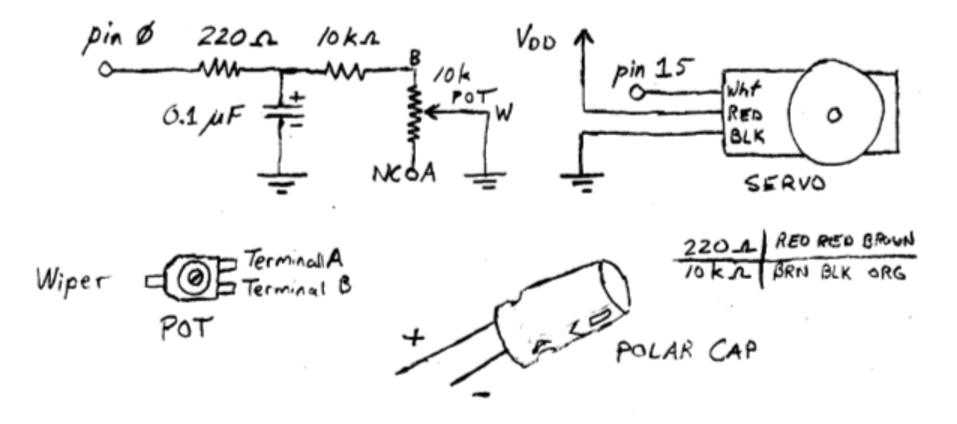
\includegraphics[width=.7\textwidth]{rudder-circuit.pdf}
\caption{Rudder Controller and Wiper Controller Circuit}
\label{rudder-circuit}
\end{figure}

\begin{figure}[ht]
\centering
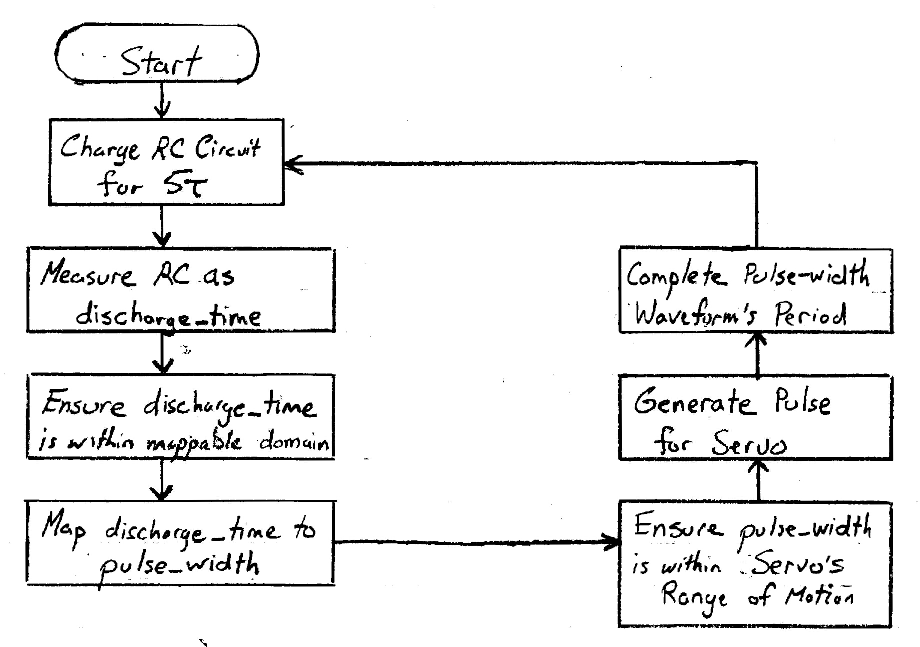
\includegraphics[width=0.5\textwidth]{rudder-flowchart.pdf}
\caption{Rudder Controller Implementation Flowchart}
\label{rudder-flowchart}
\end{figure}

\subsection{Wiper Controller}

\begin{figure}[ht]
\centering
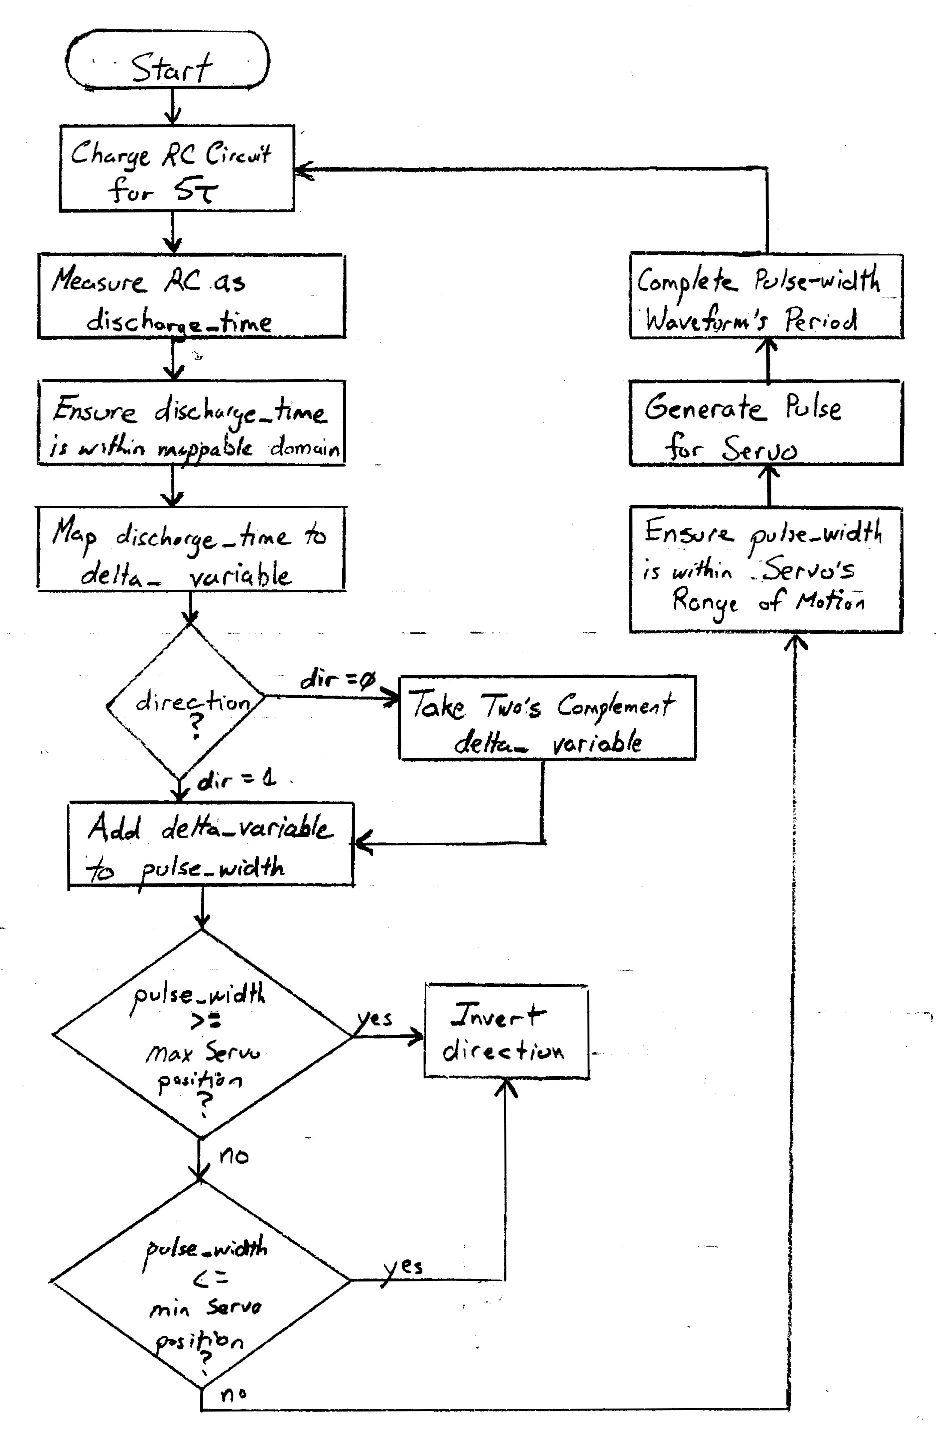
\includegraphics[width=0.5\textwidth]{wiper-flowchart.pdf}
\caption{Wiper Controller Flowchart}
\label{wiper-flowchart}
\end{figure}

\section{Expected Results}

I expected both circuits to behave according to the problem statements.

\section{Experiment and Design Revisions}

\subsection{Rudder Controller}

When I first built this project's implementation, the controller worked
for 90\% of the potentiometer's input range. However, when the discharge
time was on the lower range of its possible values, the rudder would
suddenly shift from near $45^{o}$ to the $135^{o}$ position.
After adding a \texttt{DEBUG} statement, I saw the following transition
occuring:
\begin{verbatim}
discharge_time = 622, pulse_width = 502
discharge_time = 621, pulse_width = 501
discharge_time = 620, pulse_width = 500
discharge_time = 619, pulse_width = 500
discharge_time = 618, pulse_width = 1000
\end{verbatim}

What was occuring was that the \texttt{discharge\_time} from the RC circuit
was coming back slightly lower than the minimum value I was expecting.
Thus the subraction \mbox{\texttt{(discharge\_time - MAPPING\_X1)}} resulted
in a negative number, except the variable was not declared as signed so
the result of the two's-complement arithmetic was the maximum possible
value for the 16-bit Word. Later in the code is the function
\mbox{\texttt{MAX 1000}}, so that is where the 1000 is coming from.

The fix for this bug was very simple, simply treating the
\texttt{discharge\_time} variable with \mbox{\texttt{MIN MAPPING\_X1}}
prior to calculating the \texttt{pulse\_width}.

\subsection{Wiper Controller}

When I first implemented this circuit the program worked but the servo
was extremely jerky. At first I thought this meant my speeds were too
high, but it turned out it was only due to a \texttt{DEBUG} statement
in the loop that was throwing off the pulse width timing.

Removal of the \texttt{DEBUG} statement fixed the error.

\section{Observations}

Both circuits eventually worked as expected, and photos of the working boards are shown in
\hyperref[rudder-controller]{figure \ref{rudder-controller}}
and \hyperref[wiper-controller]{figure \ref{wiper-controller}}.

\begin{figure}
\centering
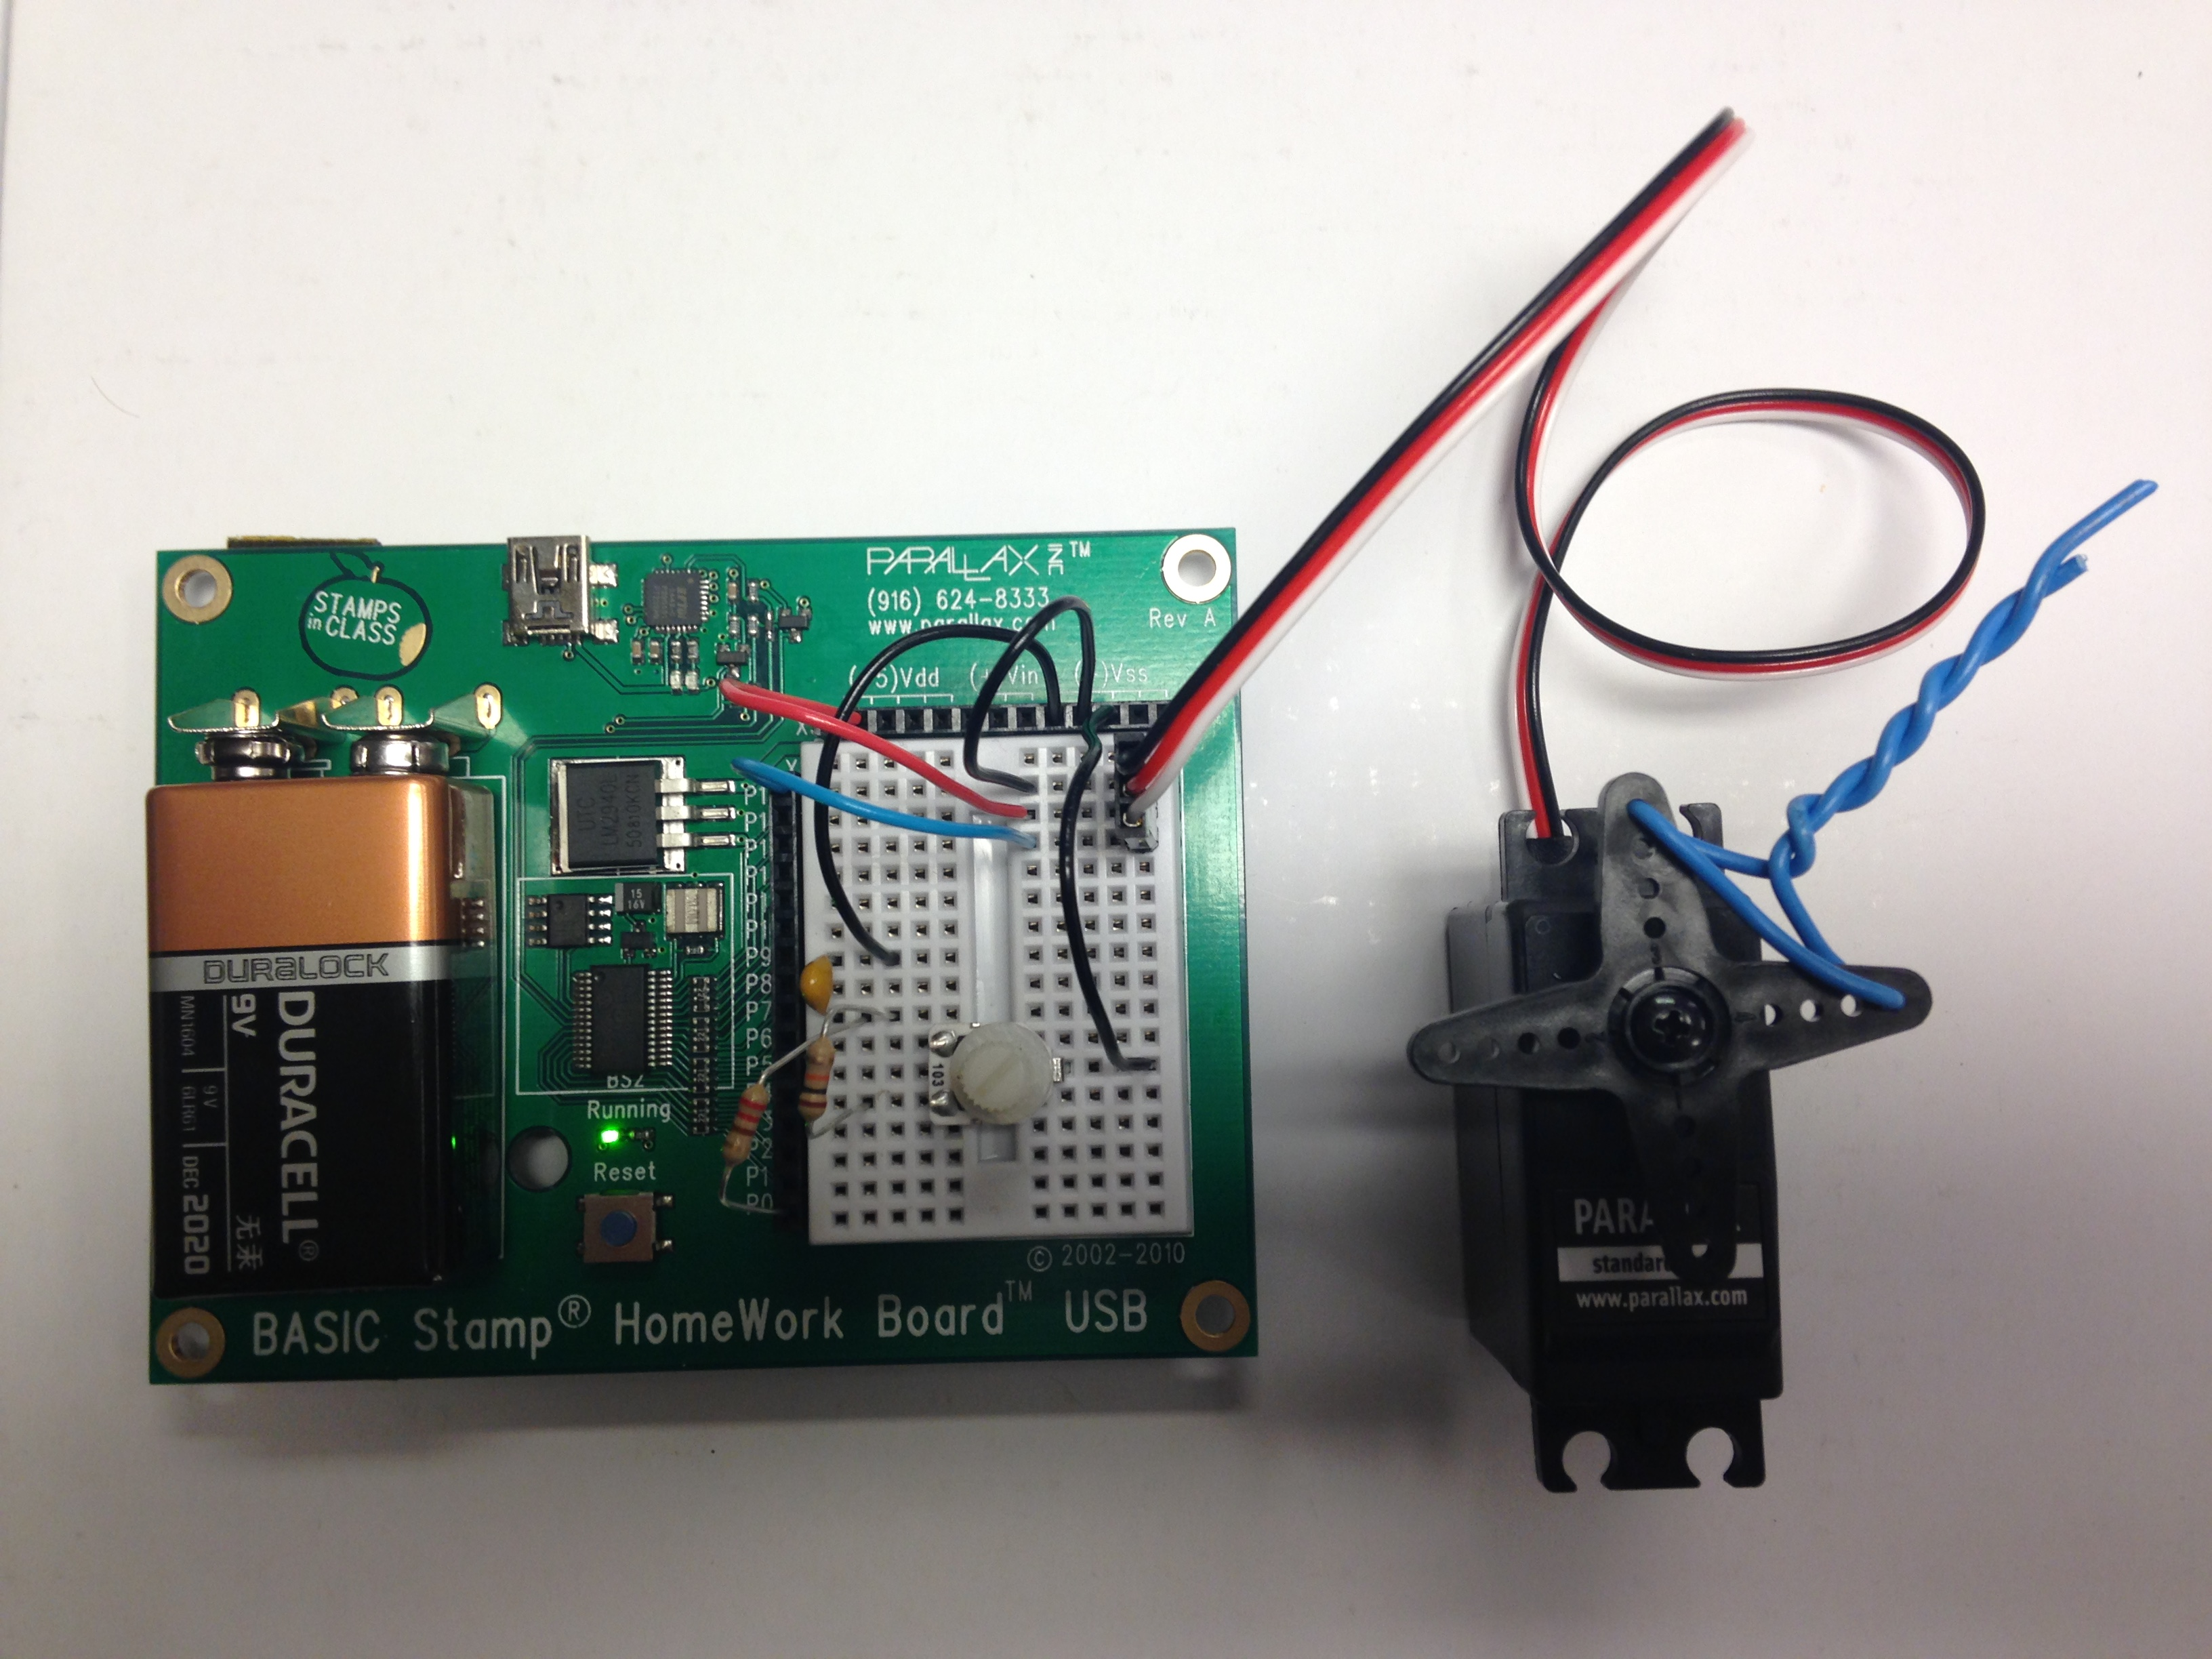
\includegraphics[width=0.6\textwidth]{rudder-controller.jpg}
\caption{Rudder Controller Board}
\label{rudder-controller}
\end{figure}

\begin{figure}
\centering
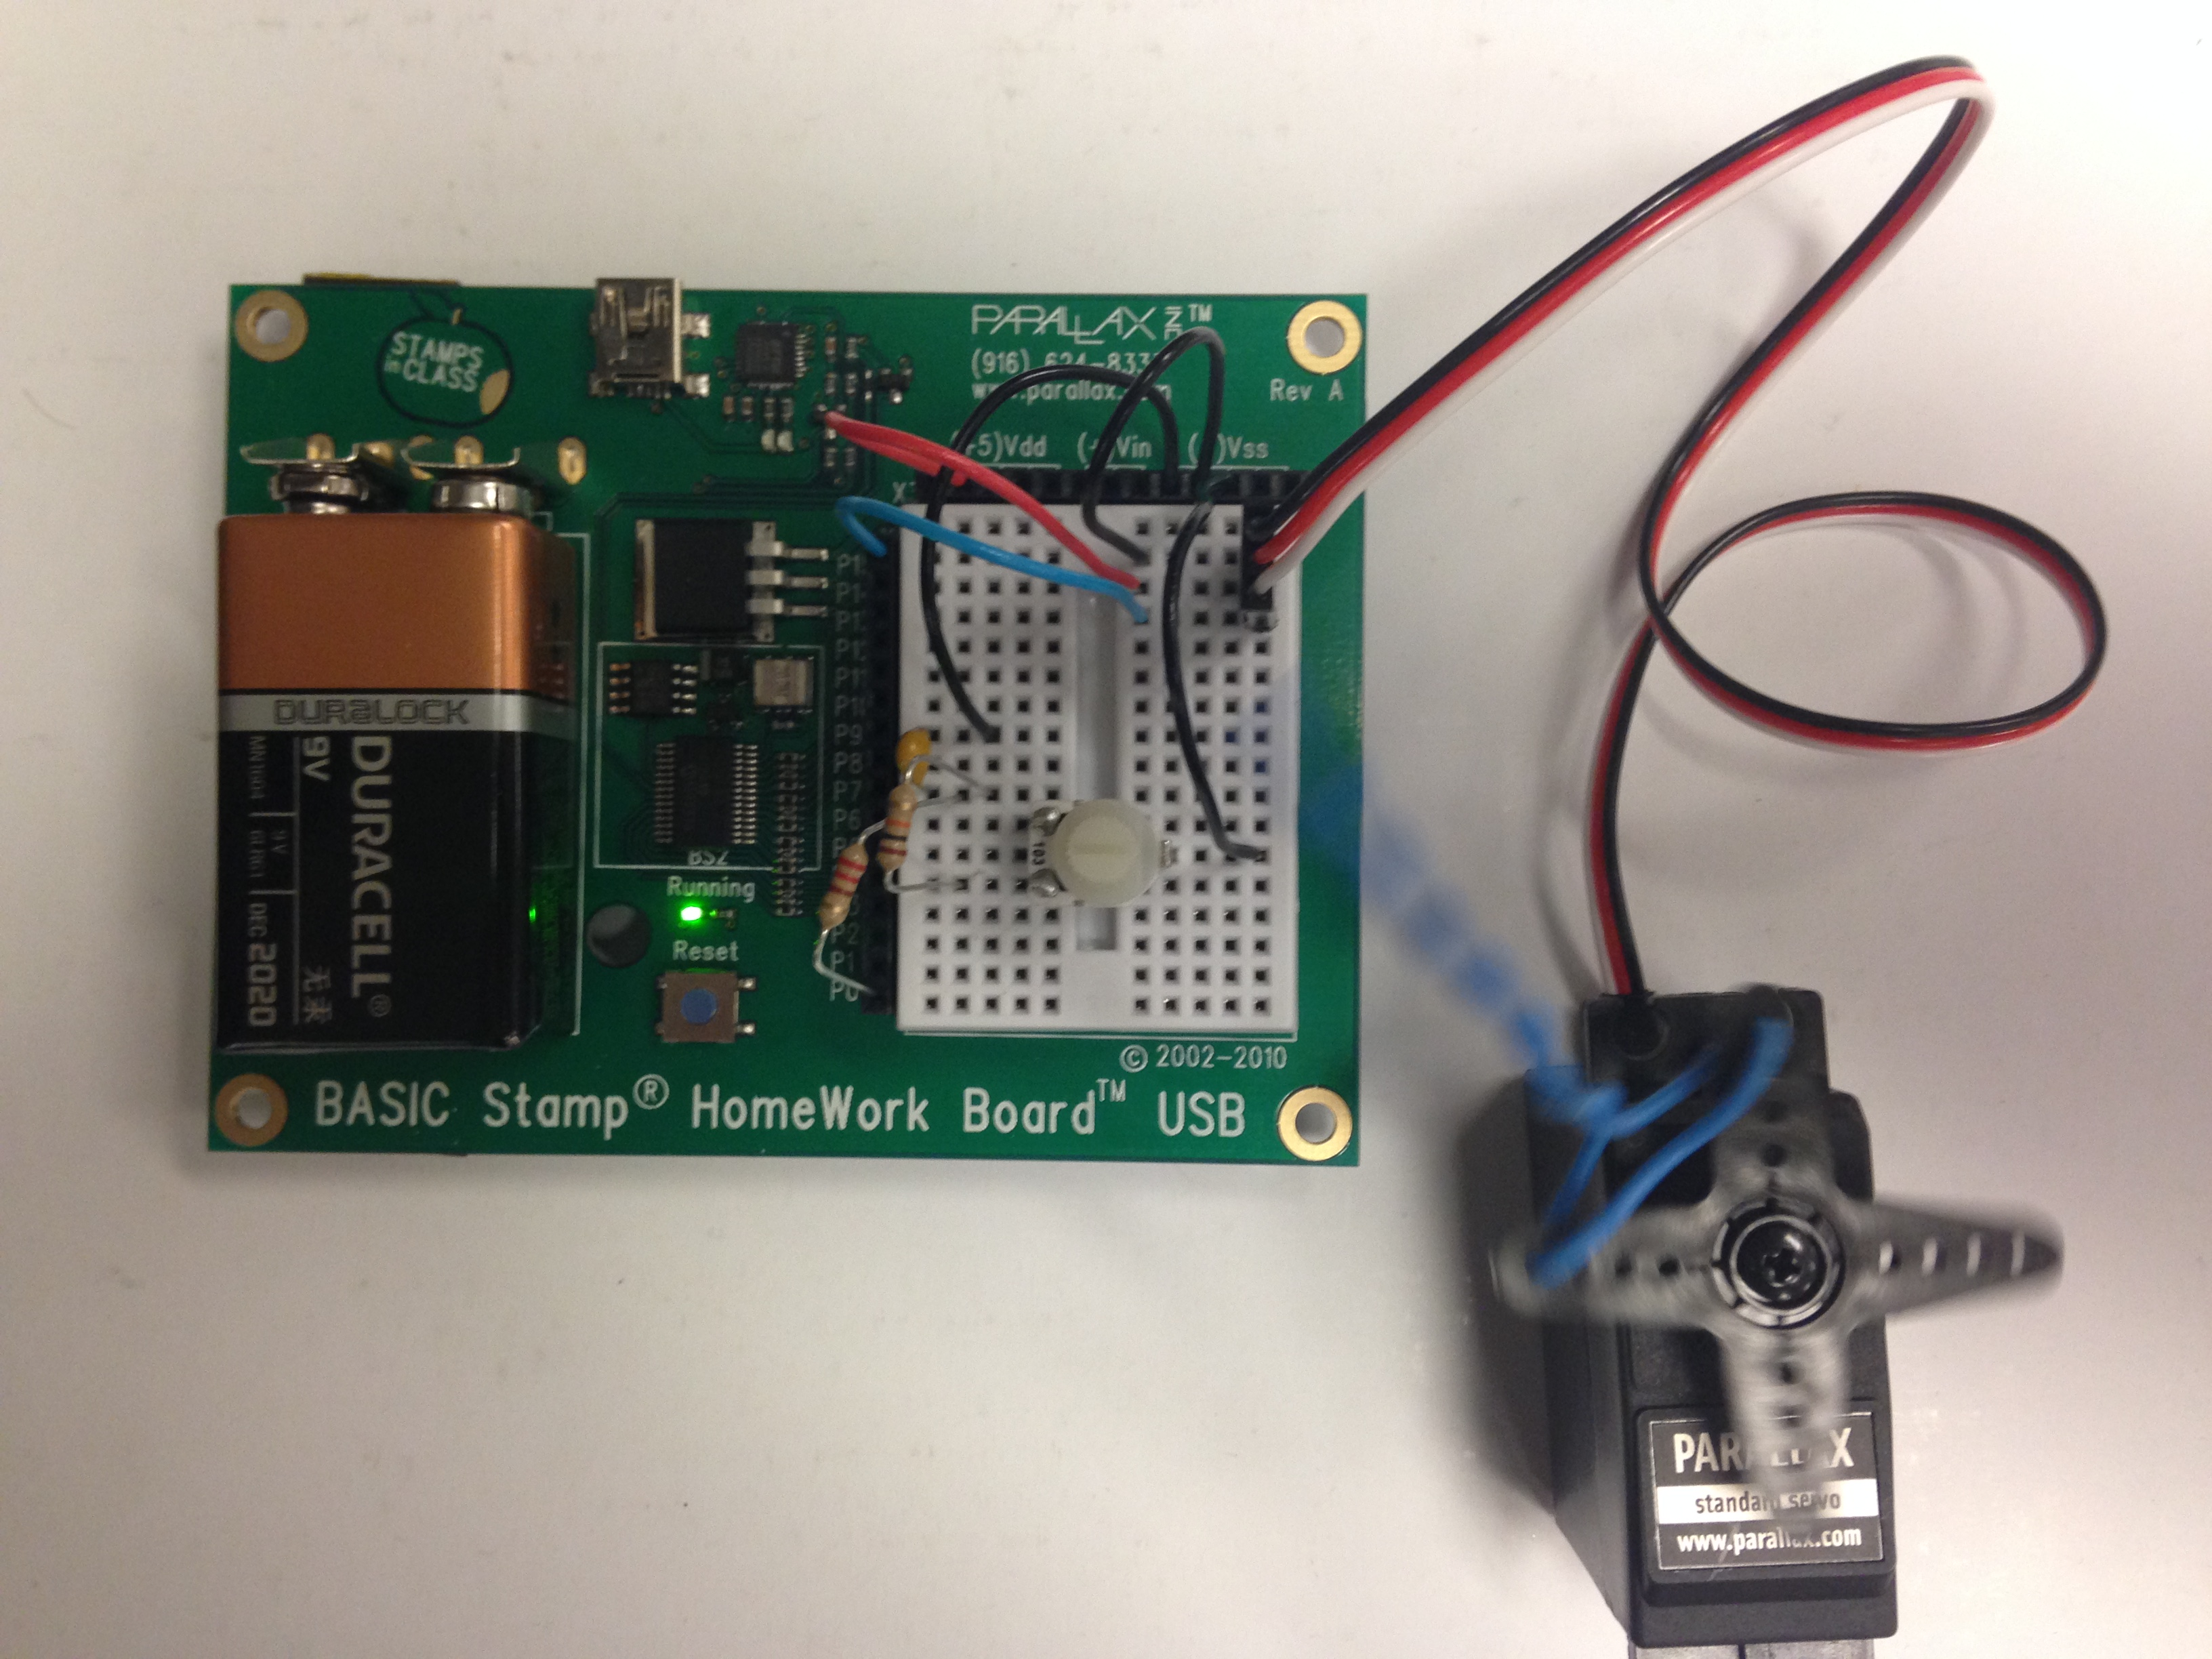
\includegraphics[width=0.6\textwidth]{wiper-controller.jpg}
\caption{Wiper Controller Board}
\label{wiper-controller}
\end{figure}

\section{Discussion}

\section{Exercises}

There were no exercises given.

\clearpage
\section{Programs}

\subsection{Rudder Controller}
\begingroup
\fontsize{11pt}{13pt}

\verbatiminput{Rudder-Controller.bs2}

\endgroup

\clearpage
\subsection{Wiper Controller}
\begingroup
\fontsize{9pt}{10pt}

\verbatiminput{Wiper-Controller.bs2}

\endgroup

\end{document}
